\section*{Examples}
This section collects ready-to-copy examples of the most common elements of a report. Delete it, together with the useful links, in your final document.

%----------------------------------------------------------------------------------------
\subsection*{Figures}

Two images side by side, each with its own sub-caption (\texttt{subfigure} environment, \cref{fig:subfigures}).
\begin{figure}[ht]
    \centering
    \begin{subfigure}{0.3\textwidth}
        \centering
        
\includegraphics[width=0.6\linewidth]{img/pictograms/acute-toxicity.png}
        \caption{Acute toxicity}
        \label{fig:acute-toxicity}
    \end{subfigure}
    \begin{subfigure}{0.3\textwidth}
        \centering
        
\includegraphics[width=0.6\linewidth]{img/pictograms/explosive.png}
        \caption{Explosive}
        \label{fig:explosive}
    \end{subfigure}
    \caption{Two sub-figures centred on the page.}
    \label{fig:subfigures}
\end{figure}

\textit{Lorem ipsum dolor sit amet, consectetur adipiscing elit. Maecenas eget nisl elementum, pretium libero suscipit, interdum tellus. Praesent luctus commodo massa, vel molestie augue laoreet ac. Phasellus sodales auctor erat eu porta. Donec at volutpat nunc. Phasellus pretium, eros vitae cursus ornare, turpis massa egestas sem, ut varius ipsum metus nec mi.}

A figure with the caption beside it (\texttt{floatrow} package, \cref{fig:caption-beside}).
\begin{figure}[ht]
    \floatbox[{\capbeside\thisfloatsetup{capbesideposition={right,center},capbesidewidth=0.45\textwidth}}]{figure}[\FBwidth]
    {\caption{Benzoic acid: a figure with its caption on the right.}\label{fig:caption-beside}}
    {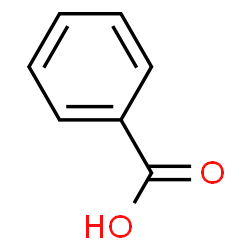
\includegraphics[width=0.15\textwidth]{img/benzoic_acid.png}}
\end{figure}

\begin{wrapfigure}{r}{0.3\textwidth}
    \centering
    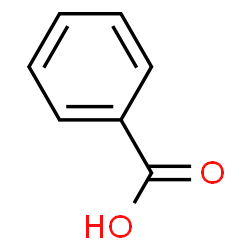
\includegraphics[width=0.2\textwidth]{img/benzoic_acid.png}
    \caption{A figure on the right, wrapped by the text.}
    \label{fig:wrapped}
\end{wrapfigure}
\textit{Nullam vel lorem porttitor, convallis ex eget, condimentum velit. Integer sed sem aliquet, elementum ipsum in, rutrum elit. Vestibulum in arcu eget odio egestas varius. Vivamus lacus augue, dignissim at arcu a, consequat iaculis leo. Nam sit amet varius tellus. Nulla tempor velit nibh, et tincidunt diam porta vel. Mauris sit amet erat ut neque vehicula ultrices et eu sem. Phasellus pellentesque ultricies sapien. Curabitur at sodales mauris, maximus auctor mi. Vestibulum semper mauris in euismod rutrum. Fusce pellentesque in mi ac euismod. Nam gravida magna ut volutpat placerat. Pellentesque habitant morbi tristique senectus et netus et malesuada fames ac turpis egestas. Sed consequat justo condimentum metus bibendum mattis. Etiam id euismod ante. Nam sit amet ex libero.}

\begin{figure}[ht]
    \centering
    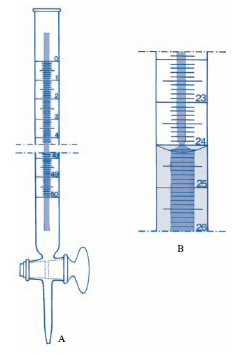
\includegraphics[height=4cm]{img/burette.jpg}
    \caption{A burette.}
    \label{fig:burette}
\end{figure}

The GHS hazard pictograms are available in \texttt{img/pictograms/} (\cref{fig:pictograms}).
\begin{figure}[ht]
    \centering
    \newcommand{\pictogram}[2]{%
        \begin{subfigure}{0.19\textwidth}
            \centering
            \includegraphics[width=0.65\linewidth]{img/pictograms/#1.png}
            \caption*{\scriptsize #1\\#2}
        \end{subfigure}}
    \pictogram{explosive}{GHS01}
    \pictogram{flammable}{GHS02}
    \pictogram{oxidizing}{GHS03}
    \pictogram{gas-under-pressure}{GHS04}
    \pictogram{corrosive}{GHS05}\\[1ex]
    \pictogram{acute-toxicity}{GHS06}
    \pictogram{health-hazard}{GHS07}
    \pictogram{serious-health-hazard}{GHS08}
    \pictogram{hazardous-to-environment}{GHS09}
    \caption{GHS pictograms: file name and code.}
    \label{fig:pictograms}
\end{figure}

%----------------------------------------------------------------------------------------
\clearpage
\subsection*{Units and cross-references}
Quantities are typeset with \texttt{siunitx} and labelled objects are referenced with \texttt{cleveref}, which adds the word (Figure, Table, Equation) automatically.
\begin{center}
    \begin{tabular}{l l}
        \toprule
        \textbf{Code}                                & \textbf{Result}                         \\
        \midrule
        \verb|\qty{25.00}{\milli\litre}|             & \qty{25.00}{\milli\litre}               \\
        \verb|\qty{9.81}{\metre\per\second\squared}| & \qty{9.81}{\metre\per\second\squared}   \\
        \verb|\qty{0.1032(4)}{\mole\per\litre}|      & \qty{0.1032(4)}{\mole\per\litre}        \\
        \verb|\num{6.022e23}|                        & \num{6.022e23}                          \\
        \verb|\ang{104.5}|                           & \ang{104.5}                             \\
        \midrule
        \verb|\cref{fig:burette}|                    & \cref{fig:burette}                      \\
        \verb|\cref{tab:reagents,tab:synthesis}|     & \cref{tab:reagents,tab:synthesis}       \\
        \verb|\cref{eq:moles}|                       & \cref{eq:moles}                         \\
        \bottomrule
    \end{tabular}
\end{center}

%----------------------------------------------------------------------------------------
\subsection*{Structural formulae}
Structural formulae are drawn with the \texttt{chemfig} package (\cref{tab:chemfig}).
\begin{table}[ht]
    \centering
    \small
    \setchemfig{atom sep=1.8em}
    \renewcommand{\arraystretch}{2.2}
    \begin{tabular}{l l c}
        \toprule
        \textbf{Feature}         & \textbf{Code}                                     & \textbf{Result}                            \\
        \midrule
        Bond angles in units of \ang{45} & \verb|\chemfig{A-[1]B-[7]C}|              & \chemfig{A-[1]B-[7]C}                      \\
        Absolute angles          & \verb|\chemfig{A-[:50]B-[:-25]C}|                 & \chemfig{A-[:50]B-[:-25]C}                 \\
        Relative angles          & \verb|\chemfig{A-[::50]B-[::-25]C}|               & \chemfig{A-[::50]B-[::-25]C}               \\
        Regular polygons         & \verb|\chemfig{A*5(-B=C-D-E=)}|                   & \chemfig{A*5(-B=C-D-E=)}                   \\
        Incomplete rings         & \verb|\chemfig{A*5(-B=C-D)}|                      & \chemfig{A*5(-B=C-D)}                      \\
        Branched molecule        & \verb|\chemfig{H-C(-[2]H)(-[6]H)-C(=[1]O)-[7]H}|  & \chemfig{H-C(-[2]H)(-[6]H)-C(=[1]O)-[7]H}  \\
        Branched ring            & \verb|\chemfig{*6(-=(-CH_3)--(=O)-=)}|            & \chemfig{*6(-=(-CH_3)--(=O)-=)}            \\
        \bottomrule
    \end{tabular}
    \caption{Some \texttt{chemfig} features.}
    \label{tab:chemfig}
\end{table}

Molecules can be named and the bond style changed (\cref{fig:ethanal}).
\begin{figure}[ht]
    \centering
    \setchemfig{atom sep=2.5em, bond style={line width=1pt, red, dash pattern=on 2pt off 2pt}}
    \chemname{\chemfig{H-C(-[2]H)(-[6]H)-C(=[1]O)-[7]H}}{Ethanal}
    \caption{Named molecule with a custom bond style.}
    \label{fig:ethanal}
\end{figure}

%----------------------------------------------------------------------------------------
\clearpage
\subsection*{Molecular orbital diagrams}
Molecular orbital diagrams are drawn with the \texttt{modiagram} package (\cref{fig:modiagram}).
\begin{figure}[ht]
    \centering
    \begin{subfigure}{0.3\textwidth}
        \centering
        \begin{modiagram}
            \atom{left}{1s, 2s, 2p}
        \end{modiagram}
        \caption{Atomic orbitals}
    \end{subfigure}
    \hfill
    \begin{subfigure}{0.3\textwidth}
        \centering
        \begin{modiagram}
            \atom{left}{1s}
            \atom{right}{1s={;up}}
            \molecule{1sMO={0.75;pair,up}}
        \end{modiagram}
        \caption{\ce{He2+}}
    \end{subfigure}
    \hfill
    \begin{subfigure}{0.3\textwidth}
        \centering
        \begin{modiagram}
            \atom{left}{1s}
            \atom{right}{1s={;up}}
            \molecule{1sMO={;pair,up}}
            \draw[<-, shorten <=8pt, shorten >=15pt, blue] (1sigma*) --++(1,1) node[above] {antibonding};
        \end{modiagram}
        \caption{Annotated orbital}
    \end{subfigure}

    \bigskip
    \begin{subfigure}{\textwidth}
        \centering
        \begin{modiagram}
            \atom{left}{1s, 2s, 2p = {;pair,up,up}}
            \atom{right}{1s, 2s, 2p = {;pair,up,up}}
            \molecule{1sMO, 2sMO, 2pMO = {;pair,pair,pair,up,up}}
        \end{modiagram}
        \caption{\ce{O2}}
    \end{subfigure}
    \caption{Examples of molecular orbital diagrams.}
    \label{fig:modiagram}
\end{figure}

%----------------------------------------------------------------------------------------
\clearpage
\subsection*{Flowchart}
A flowchart is useful for long or branched procedures (\cref{fig:flowchart}). The node and arrow styles are defined in \texttt{config/flowchart.tex}.
\begin{figure}[ht]
    \centering
    % Tutorial: https://www.overleaf.com/learn/latex/LaTeX_Graphics_using_TikZ%3A_A_Tutorial_for_Beginners_(Part_3)%E2%80%94Creating_Flowcharts
    \begin{tikzpicture}[node distance=1cm and 1.5cm]
        \node (start)  [starter] {Start};
        \node (in1)    [io, below=of start] {Input};
        \node (pro1)   [process, below=of in1] {Process 1};
        \node (dec1)   [decision, below=of pro1] {Decision 1};
        \node (pro2a)  [process, below=of dec1] {Process 2a};
        \node (pro2b)  [process, right=of dec1] {Process 2b};
        \node (out1)   [io, below=of pro2a] {Output};
        \node (pro3a)  [process, right=of out1] {Process 3a};
        \node (note)   [process_longtext2.5, right=of pro3a] {A process with a longer description.};
        \node (db)     [database, above=of note] {Data};
        \node (stop)   [terminator, below=of out1] {Stop};

        \draw [arrow_stealth] (start) -- (in1);
        \draw [arrow_stealth] (in1) -- (pro1);
        \draw [arrow_stealth] (pro1) -- (dec1);
        \draw [arrow_stealth] (dec1) -- node[anchor=east] {yes} (pro2a);
        \draw [arrow_stealth] (dec1) -- node[anchor=south] {no} (pro2b);
        \draw [arrow_stealth_rounded] (pro2b) |- (pro1);
        \draw [arrow_latex] (pro2a) -- (out1);
        \draw [line_rect] (out1) -- (pro3a);
        \draw [double_arrow_latex] (pro3a) -- (note);
        \draw [arrow_latex] (note) -- (db);
        \draw [arrow_latex_rounded] (note) |- (stop);
        \draw [arrow_latex] (out1) -- (stop);
    \end{tikzpicture}
    \caption{Example flowchart.}
    \label{fig:flowchart}
\end{figure}

%----------------------------------------------------------------------------------------
\clearpage
\subsection*{Notes}
\begin{sloppypar}
Notes are added with \verb|\unsure|, \verb|\change|, \verb|\info| and \verb|\improvement|, defined in \texttt{config/settings.tex}. The optional argument \verb|[inline]| places a note in the text instead of the margin. To hide all notes, add the \texttt{disable} option to \texttt{todonotes} in \texttt{config/package.tex}.
\end{sloppypar}

Lorem ipsum dolor sit amet, consectetur adipiscing elit. Sed eget velit ullamcorper, convallis neque eget, tempus leo. Aenean eget est ornare, mattis turpis sit amet, vestibulum ante.\unsure{Is this correct?} Integer quis molestie arcu. Duis sem felis, posuere ut ante vitae, lobortis tincidunt dolor. Ut aliquet nunc sed lorem vehicula, ac tristique velit venenatis.\change{Change this!}

Pellentesque consectetur malesuada lectus, ut faucibus diam egestas ac. Aenean porttitor at libero a venenatis. Morbi sollicitudin, leo sed pellentesque facilisis, lacus diam lobortis tellus, sit \info{This can help me in the conclusions.}amet vulputate turpis sem id ipsum. Nunc ac aliquet mi, non porta quam. Pellentesque libero nunc, \improvement{This really needs to be improved!}congue vitae mi sit amet, lobortis faucibus ante.

Sed non erat metus. Donec aliquet ex non neque sodales pretium. Aliquam eu sapien elit. Aliquam finibus felis et neque elementum, laoreet tempus urna auctor. Vivamus ac congue elit, vitae volutpat nulla.
\improvement[inline]{The following paragraph needs to be rewritten!}

Sed finibus pellentesque diam, et sagittis tortor ultrices ut. Suspendisse volutpat ullamcorper dui in cursus. Proin ullamcorper neque posuere porttitor rutrum.
\thiswillnotshow{This note is hidden because it uses the disable option.}

Finally, \verb|\listoftodos| prints the list of all notes:
\listoftodos[Notes to address]
